\documentclass[12pt]{article}
\usepackage{amsmath}
\usepackage{amssymb}
\usepackage[letterpaper,top=1in,bottom=1.25in,left=0.75in,right=0.75in,centering]{geometry}
%\usepackage{fancyhdr}
\usepackage{enumerate}
%\usepackage{lastpage}
\usepackage{multicol}
\usepackage{graphicx}

%\reversemarginpar

%\pagestyle{fancy}
%\cfoot{}
%\lhead{Math 1560}\chead{Test \# 1}\rhead{May 18th, 2017}
%\rfoot{Total: 10 points}
%\chead{{\bf Name:}}
\newcommand{\points}[1]{\marginpar{\hspace{24pt}[#1]}}
\newcommand{\skipline}{\vspace{12pt}}
%\renewcommand{\headrulewidth}{0in}
\headheight 30pt

\newcommand{\di}{\displaystyle}
\newcommand{\abs}[1]{\lvert #1\rvert}
\newcommand{\len}[1]{\lVert #1\rVert}
\renewcommand{\i}{\mathbf{i}}
\renewcommand{\j}{\mathbf{j}}
\renewcommand{\k}{\mathbf{k}}
\newcommand{\R}{\mathbb{R}}
\newcommand{\aaa}{\mathbf{a}}
\newcommand{\bbb}{\mathbf{b}}
\newcommand{\ccc}{\mathbf{c}}
\newcommand{\dotp}{\boldsymbol{\cdot}}
\newcommand{\bbm}{\begin{bmatrix}}
\newcommand{\ebm}{\end{bmatrix}}                   
\usepackage{pgf,tikz}
\usepackage{mathrsfs}
\usetikzlibrary{arrows}    
\begin{document}
\begin{center}
Math 1565 Tutorial 1 Solutions
\end{center}

\author{Instructor: Sean Fitzpatrick}

\thispagestyle{empty}
\begin{enumerate}
 \item  \textbf{Using the definition} of $\sinh(x)$, show that
 \[
 \sinh(x+y) = \sinh(x)\cosh(y)+\cosh(x)\sinh(y).
 \]
 
Starting on the right-hand side, using the definitions of $\sinh(t)$ and $\cosh(t)$, we have
\begin{align*}
\sinh(x)\cosh(y)+\cosh(x)\sinh(y) & = \left(\frac{e^x-e^{-x}}{2}\right)\left(\frac{e^y+e^{-y}}{2}\right)+\left(\frac{e^x+e^{-x}}{2}\right)\left(\frac{e^y-e^{-y}}{2}\right)\\
& = \frac{1}{4}\left(e^xe^y+e^xe^{-y}-e^{-x}e^y-e^{-x}e^{-y}\right)\\
& \quad \quad +\frac{1}{4}\left(e^xe^y-e^xe^{-y}+e^{-x}e^y-e^{-x}e^{-y}\right)\\
& = \frac{1}{4}\left(2e^{x+y}-2e^{-x-y}\right)\\
& = \frac{e^{x+y}-e^{-(x+y)}}{2} = \sinh(x+y),
\end{align*}
as required.

\bigskip

 
 \item Show that $\sin(\tan^{-1}(x)) = \dfrac{x}{\sqrt{1+x^2}}$.
 
 \bigskip
 
 We let $\theta=\tan^{-1}(x)$, which gives us $\tan\theta=x$. We can now proceed in one of two ways:
 
 \begin{enumerate}
 \item Geometric approach: we draw a little triangle, with one angle labelled by $\theta$:
 \begin{multicols}{2}
 Since $\tan\theta = x = \dfrac{x}{1}$ gives the ratio of the length of the side opposite $\theta$ to that adjacent to $\theta$, we can label two of the three sides as shown, and the Pythagorean theorem gives us the remaining side.
 \columnbreak
 \begin{center}
 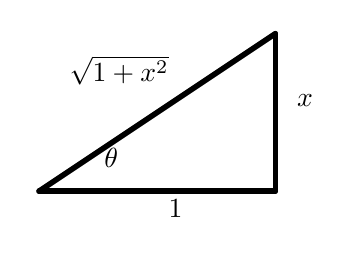
\begin{tikzpicture}[line cap=round,line join=round,>=triangle 45,x=1.0cm,y=1.0cm]
\clip(-0.14486468697728375,-0.6084778487764753) rectangle (3.491404887561501,2.0762445473783195);
%\fill[line width=2.pt] (0.,0.) -- (3.,0.) -- (3.,2.) -- cycle;
\draw [line width=2.pt] (0.,0.)-- (3.,0.);
\draw [line width=2.pt] (3.,0.)-- (3.,2.);
\draw [line width=2.pt] (3.,2.)-- (0.,0.);
\draw (3.151566609567222,1.3455922496906219) node[anchor=north west] {$x$};
\draw (1.520342875194683,0.02022296551293845) node[anchor=north west] {$1$};
\draw (0.26294124661585094,1.8383577527823247) node[anchor=north west] {$\sqrt{1+x^2}$};
\draw (0.7047310080084136,0.6659156937020663) node[anchor=north west] {$\theta$};
\end{tikzpicture}
 \end{center}
 \end{multicols}
 \end{enumerate}
\end{enumerate}
Since $\sin\theta$ gives the ratio of the lengths of the opposite side and hypotenuse, we find that
\[
\sin(\tan^{-1}(x))=\sin\theta = \dfrac{x}{\sqrt{1+x^2}}.
\]
However, we note that our solution is only valid for $x\geq 0$, since we need $0\leq \theta\leq \pi/2$ to draw the triangle. To address this, we note that both sides of our identity involve odd functions:
\[
\sin(\tan^{-1}(-x))=\sin(-\tan^{-1}(x)) = -\sin(\tan^{-1}(x))
\]
since both the $\sin$ and $\tan^{-1}$ functions are odd, and 
\[
\dfrac{-x}{\sqrt{1+(-x)^2}} = -\dfrac{x}{\sqrt{1+x^2}}.
\]
Analytic approach: From $\tan\theta=x$, we get $\sin\theta = x\cos\theta$. Now, since $\tan^2\theta+1=\sec^2\theta=1/\cos^2\theta$, we get
\[
\cos\theta = \pm\frac{1}{\sqrt{1+\tan^2\theta}}=\pm\frac{1}{\sqrt{1+x^2}}.
\]
Since $\tan^{-1}(x)\in (-\pi/2,\pi/2)$ for all $x\in \R$ and $\cos\theta>0$ for all $x$ in $(-\pi/2,\pi/2)$, we take the positive root and the result follows.
\end{document}